\documentclass[12pt,a4paper]{article}
\usepackage[russian]{babel}
\usepackage{amsmath}

\usepackage{verbatim}
\usepackage{setspace}
\singlespacing
\usepackage{graphicx}
\usepackage{caption}
\usepackage{float}
\usepackage{amsfonts}
\usepackage{amssymb}
\usepackage{graphicx}
\usepackage{subcaption}

\begin{document}


\section{Феномен Рунге}

При интерполировании полиномами больших степеней на отрезке $[-1, 1]$ возникают осциляции по краям. Процесс интерполяции расходится при данной стратегии выбора узлов (а именно стратегия - равномерная сетка).

	\begin{figure}[h!]
		\centering
		\begin{subfigure}[b]{0.4\linewidth}
			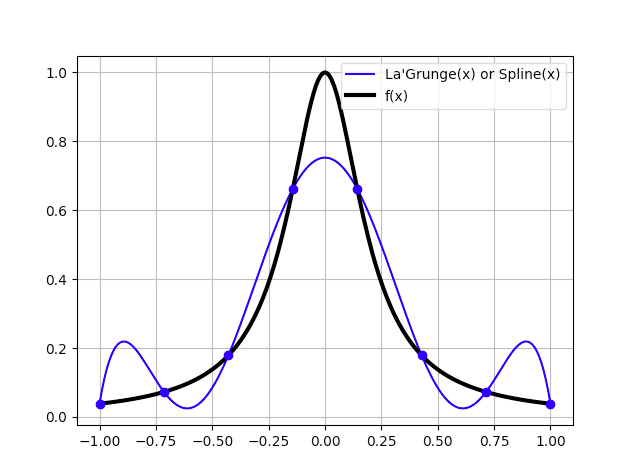
\includegraphics[width=\linewidth]{runge1}
			\caption{7 узлов.}
		\end{subfigure}
		\begin{subfigure}[b]{0.4\linewidth}
			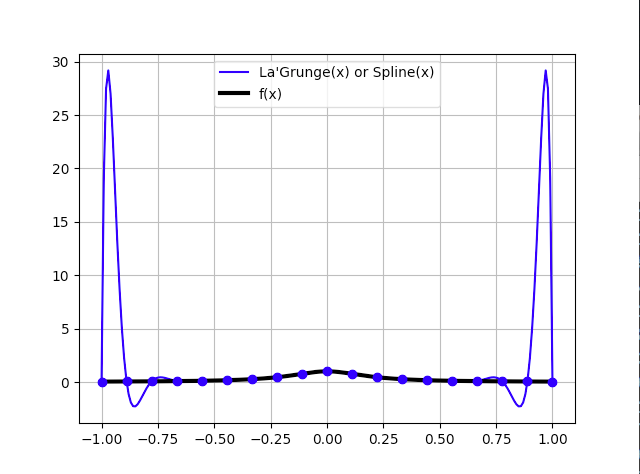
\includegraphics[width=\linewidth]{runge2}
			\caption{18 узлов.}
		\end{subfigure}
	\end{figure}

Для погрешности интерполяции имеем оценку:
\begin{equation}
||f - P_n|| \leq \frac{||f^ {(n+1)}||}{n + 1} h^{ n + 1}
\end{equation}
Норма берется в пространстве $C[-1, 1]$.

Попробуем оценить норму производной, разложив функцию в ряд
	\begin{equation}
	\begin{split}
	f(x) = \frac{1}{1 + 25x^2} = \frac{1}{(1-5ix)(1+5ix)} = \frac{1}{2(1-5ix)} + \frac{1}{2(1+5ix)} = \\ \frac{1}{2} (\sum_{k=0}^\infty(5ix)^k + \sum_{k=0}^\infty(-1)^k(5ix)^k) = \frac{1}{2}\sum_{k=0}^\infty(5^k i^k x^k (1 + (-1)^k))
	\end{split}
	\end{equation}
Видно, что при $k = 2n+1$ общий член ряда обращается в ноль. Значит суммирование надо вести по четным индексам.
\begin{equation}
f(x)  = \sum_{k=0}^\infty5^{2k} i^{2k} x^{2k}  2 = \sum_{k=0}^\infty(-1)^k5^{2k} x^{2k}.
\end{equation}
Ряд сходится при $ |5ix|< 1 \implies |x| < \frac{1}{5} $.
Степенные ряды можно почленно дифференциировать внутри круга сходимости
\begin{equation}
f^{ ' }(x) = \sum_{k=1}^\infty (-1)^k 5^{2k} 2k x^{2k-1}
\end{equation}
\begin{equation}
f^{ '' }(x) = \sum_{k=2}^\infty (-1)^k 5^{2k} 2k(2k-1) x^{2k-2}
\end{equation}
\begin{equation}
f^{ (n) }(x) = \sum_{k=n}^\infty (-1)^k 5^{2k} 2k  \ldots (2k - n + 1) x^{2k - n}
\end{equation}
Пока не понятно, что делать дальше: как оценивать модуль 
\newpage
\section{Феномен $y = 1$}
При интерполяции полиномами больших степенй возникают осцилляции по краям
\begin{figure}
	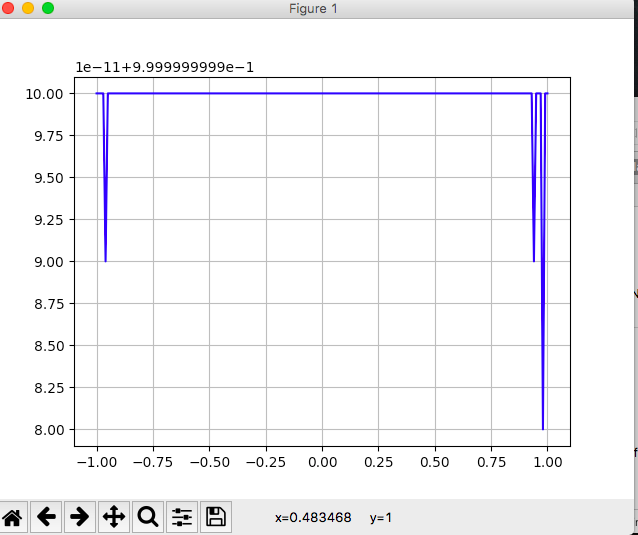
\includegraphics[width=\linewidth]{const_func.png}
	\caption{}
	\label{fig:const}
\end{figure} 

Заметим, что теоретическая оценка погрешности интерполяции - ноль, поскольку в линейном пространстве многочленов степени не выше чем $n$ $\exists!$ многочлен, проходящий через $(n+1)$ точку. Но таким многочленом (принадлежащим пространству) является линейный многочлен, тождественно равный единице.

Значения функции $f_k$ в узлах вычисляются точно (в машинной арифметике). Зато погрешность возникает при вычислении $\phi_k(x)$. \\


(Ниже идут записи, сделанные на последней лабораторной)

И вместо $\phi_k(x)$ вычисляется $\phi_k(x) + \epsilon_k$.
Дальше Вы пишете:
$$
	\sum_k f_k(\phi_k(x) + \delta\phi_k^{(n)}(x)
$$
Чем является величина  $\delta\phi_k^{(n)}(x) $ ? Почему здесь стоит она, если мы сказали, что абсолютная погрешность вычисления $\phi_k(x)$ равна $\epsilon_k$?

Далее, 
$$
\sum_k f_k(\phi_k(x) + \delta\phi_k^{(n)}(x) = \sum_k f_k \phi_k + \sum_k f_k \delta\phi_k(x)
$$
И Вы говорите, что $f_k \delta\phi_k(x) = \phi_k(x) \delta f_k$. Почему это так? Может быть, именно здесь происходит "подмена понятий": погрешность, возникающая вследствие вычислений $\phi_k(x)$ подменяется погрешностью задания значений функции (хоть у нас эта погрешность отсутсвует)
\section{Феномен $f(x) = \arctan(1 + 5x^2)}
\end{document} 